%
% einleitung.tex -- Beispiel-File für die Einleitung
%
% (c) 2020 Prof Dr Andreas Müller, Hochschule Rapperswil
%
% !TEX root = ../../buch.tex
% !TEX encoding = UTF-8
%
\subsection{Kartesisch\label{geodaeten:section:Linienelemente:Kartesisch}}
\rhead{Linienelemente Beispiele}

Wie in Abbildung [\ref{geodaeten:figure:Linienelemente:figure1}] zu sehen ist kann ein Wegstück auf einer Kurve im zweidimensionalen Kartesischen Raum mit

\begin{equation}
	\Delta s \approx \sqrt{\Delta x^2 + \Delta y^2}
\end{equation}
approximiert werden.
Durch Verkleinerung der Wegstücke bis zum Infinitesimal 

\begin{equation}
	d s = \sqrt{d x^2 + d y^2}
	%= \sqrt{\left(\frac{d x}{d t}\right)^2 \cdot d t^2 + \left(\frac{d y}{d t}\right)^2 \cdot d t^2} ,
\end{equation}
Kann das Linienelement aufgestellt werden als

\begin{equation}
 	ds^2 = \left(\dot{x}^2 +\dot{y}^2\right) %\cdot dt^2 .
 	\label{geodaeten:equation:Linienelemente:Kartesisch:equation1}
\end{equation}

%Als Vektor dargestellt entspricht das Linienelement
%\begin{equation}
%	\mathbf{d\vec{s}}^2 = \begin{pmatrix} \dot{x}^2 \\ \dot{y}^2 \end{pmatrix} = \begin{pmatrix} 1 && 0 \\ 0 && 1 \end{pmatrix} \cdot \begin{pmatrix} \dot{x}^2 \\ \dot{y}^2 \end{pmatrix} \cdot dt^2 .
%\end{equation}
%Diese Vektordarstellung ist in Aussicht auf den Metrischen Tensor (Abschnitt \ref{geodaeten:section:MetrischerTensor}) nützlich.


\begin{figure}
	\centering
	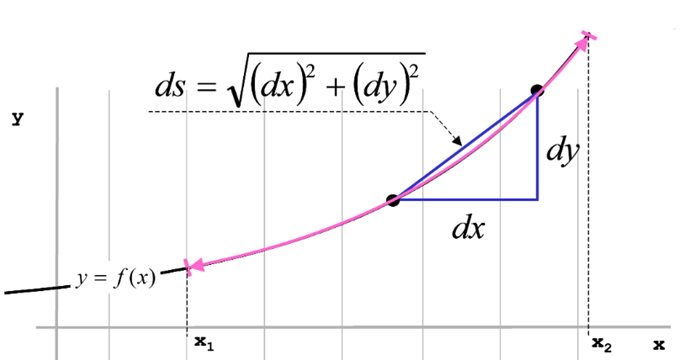
\includegraphics[width=0.7\linewidth]{papers/geodaeten/Abbildungen/Linienelemente/LinKartes1}
	\caption{Linienelement im Kartesischen Raum}
	\label{geodaeten:figure:Linienelemente:Kartesisch:figure1}
	\cite{geodaeten:kartesisch}
\end{figure}
